%%%%%%%%%%%%%%%%%%%%%%%%%%%%%%%%%%%%%%%%%
%
% Funkcionalna verifikacija hardvera
% 
%%%%%%%%%%%%%%%%%%%%%%%%%%%%%%%%%%%%%%%%%

Sedma vežba je posvećena implementaciji drajvera. Dat je pregled mogućih načina
komunikacije sa sekvencerom, klasična strukutra drajvera i opisani česti modeli
koji se sreću u praksi. Pored opisa drajvera dat je i opis konfiguracione baze
podataka i virtuelnih interfejsa.

%========================================================================================
% Section
%========================================================================================

\section{Virtuelni interfejs}

Pošto je dizajn koji se testira statička instanca, a testbenč dinamička oni se
ne mogu direktno povezati. Za povezivanje se koristi virtualni interfejs, pri
čemu je dizajn povezan na instancu ovog interfejsa u glavnom modulu. Ovo
omogućava drajveru i monitoru direktan pristup signalima dizajna koji se
verifikuje na sledeći način: povezivanje testbenča i dizajna se mora uraditi bez
dodatnih modifikacija u samom dizajnu, u vidu dodatnih konekcija ili nekih
drugih modifikacija, a zatim se informacije o konekciji prosleđuju svim
agentima kojima je potreban pristup interfejsu. Povezivanje i prosleđivanje
informacija se dešava samo u glavnom modulu kako bi se lakše reagovalo na
promene u dizajnu i poboljšala stabilnost i ponovna upotreba testbenča.\\

Interfejs se definiše u posebnoj SystemVerilog-ovoj konstrukciji istoimenog
naziva. U ovom bloku se, pored samih deklaracija portova, nalaze i sve provere
vezane za same signale. Te provere su implementirane kao tvrđenja (engl.
\emph{assertions}) i mogu biti raznolike: provere da pojedini signali nikad
nemaju nepoznatu vrednost, da su stablini u nekom intervalu, da imaju
odgovarajuće vrednosti posle reseta, ... Pisanje tvrđenja izlazi iz okvira ovog
kursa. Za dodatne informacije pogledati šesnaesto poglavlje SystemVerilog
standarda.\\

Interfejsi se prosleđuju komponentama koristeći UVM-ov mehanizam za
konfiguracije opisan u narednom poglavlju.

%========================================================================================
% Section
%========================================================================================

\section{Konfiguracioni \emph{database}}

Kao što je ranije navedeno, verifikacione komponente se kreiraju imajući u vidu
ponovnu upotrebu i konfigurabilnost. Mogu sadržati mnoge funkcionalnosti koje
nisu potrebne za svaki projekat. Pomoću UVM-ovog mehanizma za konfiguracije,
može se lako definisati potrebna konfiguracija koja će se koristiti u datom
projektu. U tipičnom testbenču postoji nekoliko konfiguracionih parametara koji
su vezani za neke komponente. UVM vodi računa i o opsegu za koji se definišu
vrednosti konfiguracionih parametara, tako da je moguće setovati vrednost samo
za neke komponente, a ne za sve koje koriste taj objekat. Na primer da li
pojedine komponente treba da vrše proveru ispravnosti ili da sakupljaju podatke
o pokrivenosti. Setovanje ovih parametara se obično vrši u samom testu, ali je
moguće definisati podrazumevane vrednosti za sve parametre ukoliko se
eksplicitno ne odredi njihova vrednost. Moguće je koristiti i konfiguracione
klase koje olakšavaju randomizaciju konfiguracionih atributa i rešavanje
zavisnosti među atributima. Olakšava se i dodavanje novih atributa ili
zavisnosti tako što se klasa nasledi i dodaju novi parametri. Željena
konfiguracija se bira samo u testu, a zatim se, pomocu UVM-ovog mehanizma,
prosledi željenim komponentama.\\

\emph{uvm\(\_\)config\(\_\)db} je UVM-ov konfiguracioni mehanizam baziran na
tipovima koji nudi mogućnost hijerarhijskog specificiranja konfiguracionih
parametara na željene vrednosti. \emph{uvm\(\_\)config\(\_\)db} može podešavati
skalarne objekte, pokazivače na klase, redove, nizove, čak i virtuelne
interfejse. Metode za setovanje odnosno preuzimanje vrednosti su
\emph{uvm\(\_\)config\(\_\)db::set} i \emph{uvm\(\_\)config\(\_\)db::get}.
Njihovi prototipi su:

\begin{lstlisting}
void uvm_config_db#(type T = int)::set(uvm_component cntxt, string inst_name, string field_name, T value);
bit uvm_config_db#(type T=int)::get(uvm_component cntxt, string inst_name, string field_name, ref T value);
\end{lstlisting}

gde je:

\begin{itemize}
\item T - tip podatka koji se prosleđuje (skalarni objekat, red, klasa,
  virtuelni interfejs, ...)
\item Cntxt - hijerarhijska putanja za koju se podešava / preuzima vrednost
\item Inst\(\_\)name - hijerarhijska putanja koja limitira pristup bazi
\item Field\(\_\)name - labela preko koje se traži unos
\item Value - vrednost koja će se upisati u bazu ili pročitati iz baze
\end{itemize}

\emph{Get} metoda vraća 1 ukoliko je vrednost uspešno preuzeta iz baze, a 0 u
suprotnom.\\

Na primer, u UVM se virtuelni interfejs uvek prosleđuje koristeći ovaj
mehanizam. U top modulu se instancira i poveže interfejs sa dizajnom koji se
verifikuje, a zatim se prosledi ostalim podkomponentama koristeći
\emph{uvm\(\_\)connfig\(\_\)db}. Primer ispod demonstrira setovanje instance
\emph{calc\(\_\)vif} u bazi uz labelu \emph{calc\(\_\)if} za globalni opseg.
Prikazan je jedino deo koda koji demonstrira \emph{config\(\_\)db}.

\lstinputlisting[caption=Primer setovanja virtualnog interfejsa, label=lst:v7_vif_config_db]{code/v7_vif_config_db.sv}

U svim komponentama u kojima želimo da koristimo taj interfejs (npr. drajver,
monitor, ...), preuzimanje iz baze bi se moglo obaviti nalik:

\begin{lstlisting}
virtual interface calc_if vif;

function void connect_phase(uvm_phase phase);
  super.connect_phase(phase);
  if (!uvm_config_db#(virtual calc_if)::get(this, "*", "calc_if", vif))
    `uvm_fatal("NO_IF",{"virtual interface must be set for: ", get_full_name(), ".vif"})
endfunction : connect_phase
\end{lstlisting}

U primeru \emph{vif} preuzima vrednost iz baze koristeći labelu \emph{calc\(\_\)if}.
Takođe se, kao dobra praksa, vrši provera uspešnosti dodele i javlja
\emph{fatal} i zaustavlja simulacija ukoliko preuzimanje nije uspešno.\\

U nastavku je dato još par primera korišćenja konfiguracione baze:

\begin{lstlisting}
uvm_config_db#(int)::set(this,"*.masters[0]", "master_id", 0);
uvm_config_db#(uvm_object_wrapper)::set(this,
                                        "*.ubus0.masters[0].sequencer.main_phase",
                                        "default_sequence",
                                        read_modify_write_seq::type_id::get());
\end{lstlisting}

Prvi primer postavlja int vrednost za \emph{master\(\_\)id} polje svih master
komponenti u okruženju čije se ime instance završava sa \emph{masters[0]}. U
drugom primeru se govori \emph{masters[0].sequencer}-u da izvrši sekvencu tipa
\emph{read\(\_\)modify\(\_\)write\(\_\)seq} kada uđe u \emph{main} fazu.\\

U i jednoj od narednih vežbi ćemo se takođe povetiti korišćenju konfiguracija i
uočiti prednosti korišćenja ovog mehanizma.\\

Ipak postoje neki parametri koji moraju biti poznati u vreme kompajliranja, na
primer širina magistrale. Ovakvi parametri se ne mogu implementirati kao
konfiguracije, već se moraju proglasiti za klasične parametre koristeći ključnu
reč \emph{parameter}. Na primer u interfejsu definišemo širinu magistrale za
podatke:

\begin{lstlisting}
parameter DATA_WIDTH = 32;
\end{lstlisting}

%========================================================================================
% Section
%========================================================================================

\section{Drajver}

U ovom poglavlju je dat opis drajvera u UVM-u. Dat je pregled klasične strukture
i sadržaja, objašnjen API i opisani česti načini korišćenja.

% ----------------------------------------------------------------------------------------

\subsection{Struktura}

Kao i sve komponente unutar UVM verifikacionog okruženja, i drajver se
implementira tako što se nasledi \emph{uvm\(\_\)driver} klasa, parametrizovana
tipom \emph{sequence item}-a koji će se koristiti za zahtev odnosno odgovor.
Pored ovog drajver treba da sadrži kod za \emph{factory} registraciju,
konstruktor, kao i virtuelni interfejs preko koga će generisati signale. Kostur
većine drajvera je dat ispod.

\begin{lstlisting}
class example_driver extends uvm_driver#(example_seq_item);

  `uvm_component_utils(example_driver)

  virtual interface example_if vif;

  function new(string name = "example_driver", uvm_component parent = null);
    super.new(name,parent);
  endfunction

  function void connect_phase(uvm_phase phase);
    super.connect_phase(phase);
    if (!uvm_config_db#(virtual example_if)::get(this, "*", "example_if", vif))
      `uvm_fatal("NO_IF",{"virtual interface must be set for: ",get_full_name(),".vif"})
  endfunction : connect_phase

  task main_phase(uvm_phase phase);
    forever begin
      seq_item_port.get_next_item(req);
      drive_tr();
      seq_item_port.item_done();
    end
  endtask : main_phase

  task drive_tr();
    // do actual driving here
    // ...
  endtask : drive_tr

endclass : example_driver
\end{lstlisting}

Nasleđivanjem \emph{uvm\(\_\)driver} klase, nasleđuje se i TLM port za
komunikaciju sa sekvencerom (\emph{seq\(\_\)item\(\_\)port}), ali i \emph{req} i
\emph{rsp} objekti koji se mogu koristiti za generisanje stimulusa. Ovi objekti
će poprimiti tip kojim je parametrizovan drajver (\emph{example\(\_\)seq\(\_\)item} u
primeru).

% ----------------------------------------------------------------------------------------

\subsection{API}

API za komunikaciju sa sekvencerom je:

\begin{itemize}
\item \emph{get\(\_\)next\(\_\)item} - blokirajuća metoda koja čeka da REQ transakcija postane dostupna i vraća pokazivač na taj objekat; nakon izvršavanja ove metode obavezno je pozvati \emph{item\(\_\)done} pre sledećeg poziva \emph{get\(\_\)next\(\_\)item}
\item \emph{try\(\_\)next\(\_\)item} - neblokirajuća metoda koja proverava da li
  postoji transakcija. Vraća \emph{null} ukoliko nema dostupne transakcije u
  sekvenceru
\item \emph{item\(\_\)done} - neblokirajuća metoda koja finalizira
  \emph{handshake} sa sekvencerom; treba je pozvati nakon
  \emph{get\(\_\)next\(\_\)item} ili uspešnog \emph{try\(\_\)next\(\_\)item};
  moguće joj je proslediti RSP transakciju kao argument
\item \emph{peek} - blokirajuća metoda koja čeka na dostupnu REQ transakciju od
  sekvencera i vraća pokazivač na taj objekat; naredni pozivi ka \emph{peek} pre
  \emph{get} ili \emph{item\(\_\)done} poziva će vratiti pokazivač na isti REQ
  objekat
\item \emph{get} - blokirajuća metoda koja čeka na dostupnu REQ transakciju od
  sekvencera; kada primi transakciju kompletira \emph{handshake} i vraća
  pokazivač na REQ objekat
\item \emph{put} - neblokirajuća metoda koja vraća RSP transakciju kao odgovor
  sekvenceru; može se pozvati u bilo kom trenutku i nije deo \emph{handshake}-a
  između drajvera i sekvencera
\end{itemize}

Na osnovu ovih metoda, postoje dva načina da se ostvari komunikacija sa
sekvencerom - koristeći \emph{get\(\_\)next\(\_\)item / item\(\_\)done} ili
\emph{get / put} mehanizam.

\subsubsection{\emph{Get\(\_\)next\(\_\)item / item\(\_\)done}}

Ovaj mehanizam omogućava drajveru da uzme transakciju od sekvencera iz sekvenci,
da je procesira i zatim kompletira rukovanje koristeći \emph{item\(\_\)done}.
Nije preporučeno proleđivanje argumenata uz \emph{item\(\_\)done}. Ovaj način
komunikacije je preferiran i čest u praksi jer obezbeđuje jasno odvajanje
između drajvera i sekvence.\\

Odgovarajuća implementacija sekvence bi sadržala \emph{start\(\_\)item} /
\emph{finish\(\_\)item} pozive, objašnjene na prethodnim vežbama. Pošto i
drajver i sekvence imaju pokazivač na isti objekat, bilo koje promene unutar
drajvera će biti vidljive i u sekvenci. Odnosno kada se pokazivač na transakciju
prosledi \emph{finish\(\_\)item} pozivu, \emph{get\(\_\)next\(\_\)item} u
drajveru će vratiti pokazivač na isti objekat. Kada se u sekvenci odblokira
\emph{finish\(\_\)item} (pozivom \emph{item\(\_\)done} u drajveru), u sekvenci
se može pristupati objektu i videti sve promene koje su načinjene u drajveru.

\begin{lstlisting}
// main faza u drajveru
task main_phase( uvm_phase phase );
  forever begin
    seq_item_port.get_next_item(req); // blokirajuci poziv koji vraca sl. transackiju
    // ... drajvovanje ...
    // na primer
    @(posedge vif.clk);
    vif.addr = req.address; // vif je virtualni interfejs
    // itd
    if(req_item.read_or_write == READ) begin // postaviti polja za odgovor
      req.rdata = vif.rdata;
    end
    seq_item_port.item_done(); // javiti sekvenceru da je zavrsena transakcija
  end
endtask : main_phase
\end{lstlisting}

\subsubsection{\emph{Get / put}}

Koristeći ovaj model, u drajveru se poziva \emph{get} metoda koja preuzima
sledeću transakciju i odmah završava rukovanje (pre nego što drajver može
procesirati transakciju). U drajveru se zatim poziva \emph{put} metoda kako bi
se označilo da je završeno sa datom transakcijom i da se vrati odgovor.Tada je u
sekvenci potrebno pozvati \emph{get\(\_\)responese} nakon
\emph{finish\(\_\)item} koji će blokirati do god se u drajveru ne pozove
\emph{put}. Mana ovog modela je što će implementacija drajvera biti
komplikovanija i što se u sekvenci mora posebno procesirati odgovor. Takođe
problemi mogu nastati ukoliko se koristi više sekvenci, a transackije nisu
ispravno označene. Više o ovoj problematici se može naći u ``UVM Cookbook''-u, u
poglavlju o sekvencama.

\begin{lstlisting}
// main faza u drajveru
task main_phase( uvm_phase phase );
  forever begin

    // uzima se sl. transakcija iz sekvencera
    seq_item_port.get(req);
 
    // ... drajvovanje ...
    // na primer
    @(posedge vif.clk);
    vif.addr = req.address; // vif je virtualni interfejs
    // itd
    if(req_item.read_or_write == READ) begin // postaviti polja za odgovor
      req.rdata = vif.rdata;
    end

    // odgovor se vraca sekvenceru
    seq_item_port.put(req);

  end
endtask : main_phase

// body task u sekvenci
virtual task body();
  example_it = example_seq_item::type_id::create("example_it");

  start_item(example_it);
  example_it.randomize();
  finish_item(example_it);

  get_response(tx); // blokirajuci poziv koji ceka da drajver vrati odgovor
endtask : body
\end{lstlisting}

% ----------------------------------------------------------------------------------------

\subsection{\emph{Use} modeli}

Ispravno generisanje stimulusa u UVM-u zavisi od dobre veze između sekvenci i
drajvera. Sekvence i drajver se moraju usaglasiti kako ne bi došlo do
\emph{deadlock} situacija kada se jedna strana zauvek blokira čekajući na
odgovor. Kako bi se izbegle ovakve situacije i omogućila laka upotreba, ako i
ponovna upotreba drajvera potrebno je dobro izmodelovati i dokumentovati
funkcionalnost drajvera. Postoji veliki broj modela za generisanje stimulusa,
međutim neki od najčešće korišćenjih modela za drajvere su:

\begin{itemize}
\item \emph{Unidirectional Non-Pipelined} - zahtevi se šalju drajveru, ali se ne
  primaju odgovori od drajvera; drajver može koristiti neki vid rukovanja, ali
  je proces slanja podataka uvek u jednom smeru; ovaj model se koristi za
  jednostrane komunikacione kanale nalik PCM interfejsu
\item \emph{Bidirectional Non-Pipelined} - podaci se šalju u oba smera,
  sekvencer šalje transakcije drajveru, dok drajver šalje odgovor; uvek je samo
  jedna transakcija aktivna, odgovor se uvek šalje pre slanja sledeće
  transakcije; ovaj model se koristi za jednostavnije protokole npr. APB
\item \emph{Pipelined} - podaci se šalju u oba smera, ali se faza slanja zahteva
  preklapa sa fazom slanja odgovora na prethodni zahtev; protočna obrada
  omogućava bolje performanse, ali komplikuje sam kod jer se zahtevi i odgovori
  moraju posebno obrađivati; primer upotrebe bio bi za AHB protokol
\item \emph{Out Of Order Pipelined} - u nekim primenama odgovori se ne šalju u
  redosledu u kom su primeljni zahtevi; ovo rezultuje u dosta komplikovanijem
  modelu gde se uglavnom koriste redovi za praćenje odgovora; još jedna
  varijacija bila bi \emph{burst} transferi za više transakcija istovremeno;
  primer upotebe npr. AXI
\end{itemize}

U nastavku je su data dva primera modela drajvera. Za kompletan opis svih modela
kao i alternativne implementacije datih modela pogledati ``UVM Cookbook'',
poglavlje ``\emph{Driver/Use Models}''.

\subsubsection{\emph{Unidirectional Non-Pipelined}}

Kod ovog modela drajver kontroliše flow koristeći \emph{get\(\_\)next\(\_\)item}
poziv kako bi primio sledeću transakciju, a poziv \emph{item\(\_\)done} metode
se vrši tek kada je završeno sa procesiranjem transakcije.\\

U nastavku je dat korišćenja ovog modela i odgovarajuće sekvence. U primeru se
šalju ADPCM paketi koristeći PCM protokol.\\

\begin{figure}[h!]
  \center
  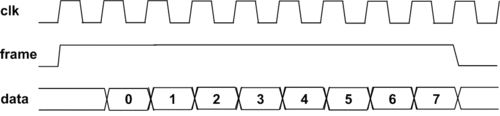
\includegraphics[width=80mm, scale=0.5]{img/v7_unidir_protocol.png}
  \caption{Protokol}
  \label{fig:unidir_protocol}
\end{figure}

\lstinputlisting[caption=Primer \emph{use} modela, label=lst:v7_unidir_driver]{code/v7_unidir_driver.sv}

\subsubsection{\emph{Bidirectional Non-Pipelined}}

Najčešće korišćen model je upravo bidirekcioni. Sekvencer šalje zahteve drajveru
koji ih izvršava, a zatim šalje odgovor nazad. Nova transakcija ne može biti
započeta do god se ne primi odgovor i ne završi prethodna. Ovi modeli se koriste
za jednostavnije protokole kao što je npr. AMPA APB.\\

Drajver prima transakciju, po protokolu koji se implementira pošalje podatke uz
eventualno čekanje i zatim postavi polja u transakciji koja služe za odgovor i
završi rukovanje sa sekvencerom. Pošto se i u drajveru i u sekvenci koristi
pokazivač na isti objekat, nakon što se sekvenca odblokira (posle
\emph{finish\(\_\)item}) može koristiti objekat sa novim vrednostima i vršiti
dalju analizu. Primer je dat ispod:

\begin{figure}[h!]
  \center
  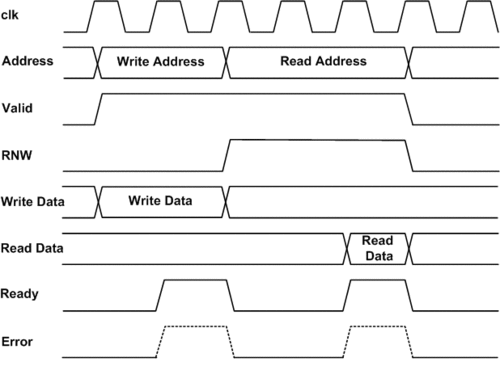
\includegraphics[width=80mm, scale=0.5]{img/v7_bidir_protocol.png}
  \caption{Protokol}
  \label{fig:bidir_protocol}
\end{figure}

\lstinputlisting[caption=Primer \emph{use} modela, label=lst:v7_bidir_driver]{code/v7_bidir_driver.sv}

%========================================================================================
% Section
%========================================================================================

\section{Zadaci}

\paragraph{Zadatak}

Implementirati drajver za primer ``Cacl1'' dizajna. Proveriti rad drajvera
koristeći sekvence razvijene na prethodnim vežbama. Pogledati \emph{waveform}-e.
Da li se DUV ponaša kao što je očekivano?

%========================================================================================
% Section
%========================================================================================

\section{Appendix}

\lstinputlisting[caption=calc\(\_\)if, label=lst:calc_if]{code/calc_if.sv}
\lstinputlisting[caption=v7\(\_\)calc\(\_\)sequencer, label=lst:v7_sequencer]{code/v7_calc_sequencer.sv}
\lstinputlisting[caption=v7\(\_\)calc\(\_\)driver, label=lst:v7_driver]{code/v7_calc_driver.sv}
\lstinputlisting[caption=v7\(\_\)calc\(\_\)seq\(\_\)item, label=lst:v7_seq_item]{code/v7_calc_seq_item.sv}
\lstinputlisting[caption=v7\(\_\)calc\(\_\)agent\(\_\)pkg, label=lst:v7_calc_agent_pkg]{code/v7_calc_agent_pkg.sv}
\lstinputlisting[caption=v7\(\_\)test\(\_\)base, label=lst:v7_test_base]{code/tests/v7_test_base.sv}
\lstinputlisting[caption=v7\(\_\)test\(\_\)simple, label=lst:v7_test_simple]{code/tests/v7_test_simple.sv}
\lstinputlisting[caption=v7\(\_\)test\(\_\)simple\(\_\)2, label=lst:v7_test_simple_2]{code/tests/v7_test_simple_2.sv}
\lstinputlisting[caption=v7\(\_\)calc\(\_\)test\(\_\)pkg, label=lst:v7_calc_test_pkg]{code/tests/v7_calc_test_pkg.sv}
\lstinputlisting[caption=v7\(\_\)calc\(\_\)base\(\_\)seq, label=lst:v7_calc_base_seq]{code/sequences/v7_calc_base_seq.sv}
\lstinputlisting[caption=v7\(\_\)calc\(\_\)simple\(\_\)seq, label=lst:v7_calc_simple_seq]{code/sequences/v7_calc_simple_seq.sv}
\lstinputlisting[caption=v7\(\_\)calc\(\_\)seq\(\_\)pkg, label=lst:v7_calc_seq_pkg]{code/sequences/v7_calc_seq_pkg.sv}
\lstinputlisting[caption=v7\(\_\)calc\(\_\)test\(\_\)pkg, label=lst:v7_calc_test_pkg]{code/v7_calc_test_pkg.sv}
\lstinputlisting[caption=v7\(\_\)calc\(\_\)verif\(\_\)top, label=lst:v7_calc_verif_top]{code/v7_calc_verif_top.sv}


%========================================================================================

